\documentclass[a4paper]{article}

%% Language and font encodings
\usepackage[english]{babel}
\usepackage[utf8x]{inputenc}
\usepackage[T1]{fontenc}

%% Sets page size and margins
\usepackage[a4paper,top=3cm,bottom=2cm,left=3cm,right=3cm,marginparwidth=1.75cm]{geometry}

%% Useful Packages

\usepackage{graphicx} % To include/embedd pdf and other graphics in the doc
\usepackage{blindtext}
\usepackage{authblk}
\usepackage{amsmath}
\usepackage{ tipa }




\title{Production Analysis of Oilfield Data}

\author{RaviKumar, Arjun\thanks{aravikumar@tamu.com}}
\author{Podhoretz, Seth\thanks{sbpodhoretz@gmail.com}}
\author{Kou, Rui\thanks{kourui.pete@tamu.edu}}
\author{Feng, Gan\thanks{fenggan@tamu.edu}}
\author{Gupta, Vivek\thanks{vivek235@tamu.edu}}
\affil{Department of Statistics, Texas A \& M University}



\begin{document}
	\maketitle
	

	
\begin{abstract}
	Our project aims to utilize the abundance of oilfield data to arrive at conclusions on the physical and
	economic aspects of the flow of hydrocarbon in the reservoir. Physical aspects that we aim to analyze include
	the prevailing flow regime (the character of flow with respect to geometry and pressure drop), interference
	between wells, and communication between wells. Economic aspects include forecasting of production rates
	into the future, and estimating the ultimate hydrocarbon recovery volumes. 
	
	
	The fluid that is of interest resides in pores of rock, several thousands of feet under the surface. As this
	fluid flows through the rock and into the well, the pressure in the rock drops, and the production rate drops.
	The nature of the production rate drop, and the backpressure held at the well together carry information on
	the physics of the process: the flow regime, possible interaction with another well, presence of boundaries
	in the reservoir. With these physical characteristics in mind, we can forecast the production rate into the
	future, thus calculating the economic life of the well, and the economics of production.
	
	
	Our dataset at the moment consists of 60 wells from the Bakken. The Bakken is a shale play in North
	Dakota, and one of the largest oil developments in recent history. It helped start the shale boom in the
	United States, reversing decades of declining US oil production volumes. 
\end{abstract}

\newpage
\section{Introduction}
 Some Introduction to be filled by subject matter experts on the problem (Arjun et al.?)
 
\section{Data Description}
 Dataset presented consists of 60 distinct wells in the <> area. The dataset has information about Monthly averages of Oil ( in bbl) , Gas ( in mcf, Thousand Cubic Feet) and Water ( in bbl , barrels). There is also information about  Daily production of these quantities. We are interested in modeling the stochastic processes , Monthly Average of Gas , Oil and Water.
 
 Density plots of these quantities as shown in Figure \ref{fig1:DensityTS} indicates high variance and right skewed distribution in data. Similar are the observations from time series plot as shown in Figure \ref{fig1:TS}. 
 
 Sample data summary statistics for a selected well is shown below as well. It is clear from the sample summary that the data has great deal of variance in it for all the three processes that are of interest to model and forecast. 
 
 \begin{center}
 	\begin{tabular}{||c c c c c c c c c ||} 
 		\hline
 		Process & Min. & 1st Qu. & Median & Mean & 3rd Qu. & Max. & Kurtosis & Skewness \\ [0.5ex] 
 		\hline\hline
 		Avg. Gas(bbl)  &  4.00   &  14.00   &  19.00  &   29.19  &  31.00   & 204.00 & 9.63 & 3.02   \\ 
 		\hline
 		Avg. Oil(mcf) &  9.32   &  26.00   &  37.00   &  75.74    & 76.50  &  642.00  & 10.01  & 3.03 \\
 		\hline
 		Avg. Water(bbl)  & 2.00    &   6.00    &   9.00   &   11.37    &  12.75   &   60.00   & 10.2  &  1.96  \\
 		\hline
 		
 		
 	\end{tabular}
 \end{center}

 \begin{figure}
 	\centering
 	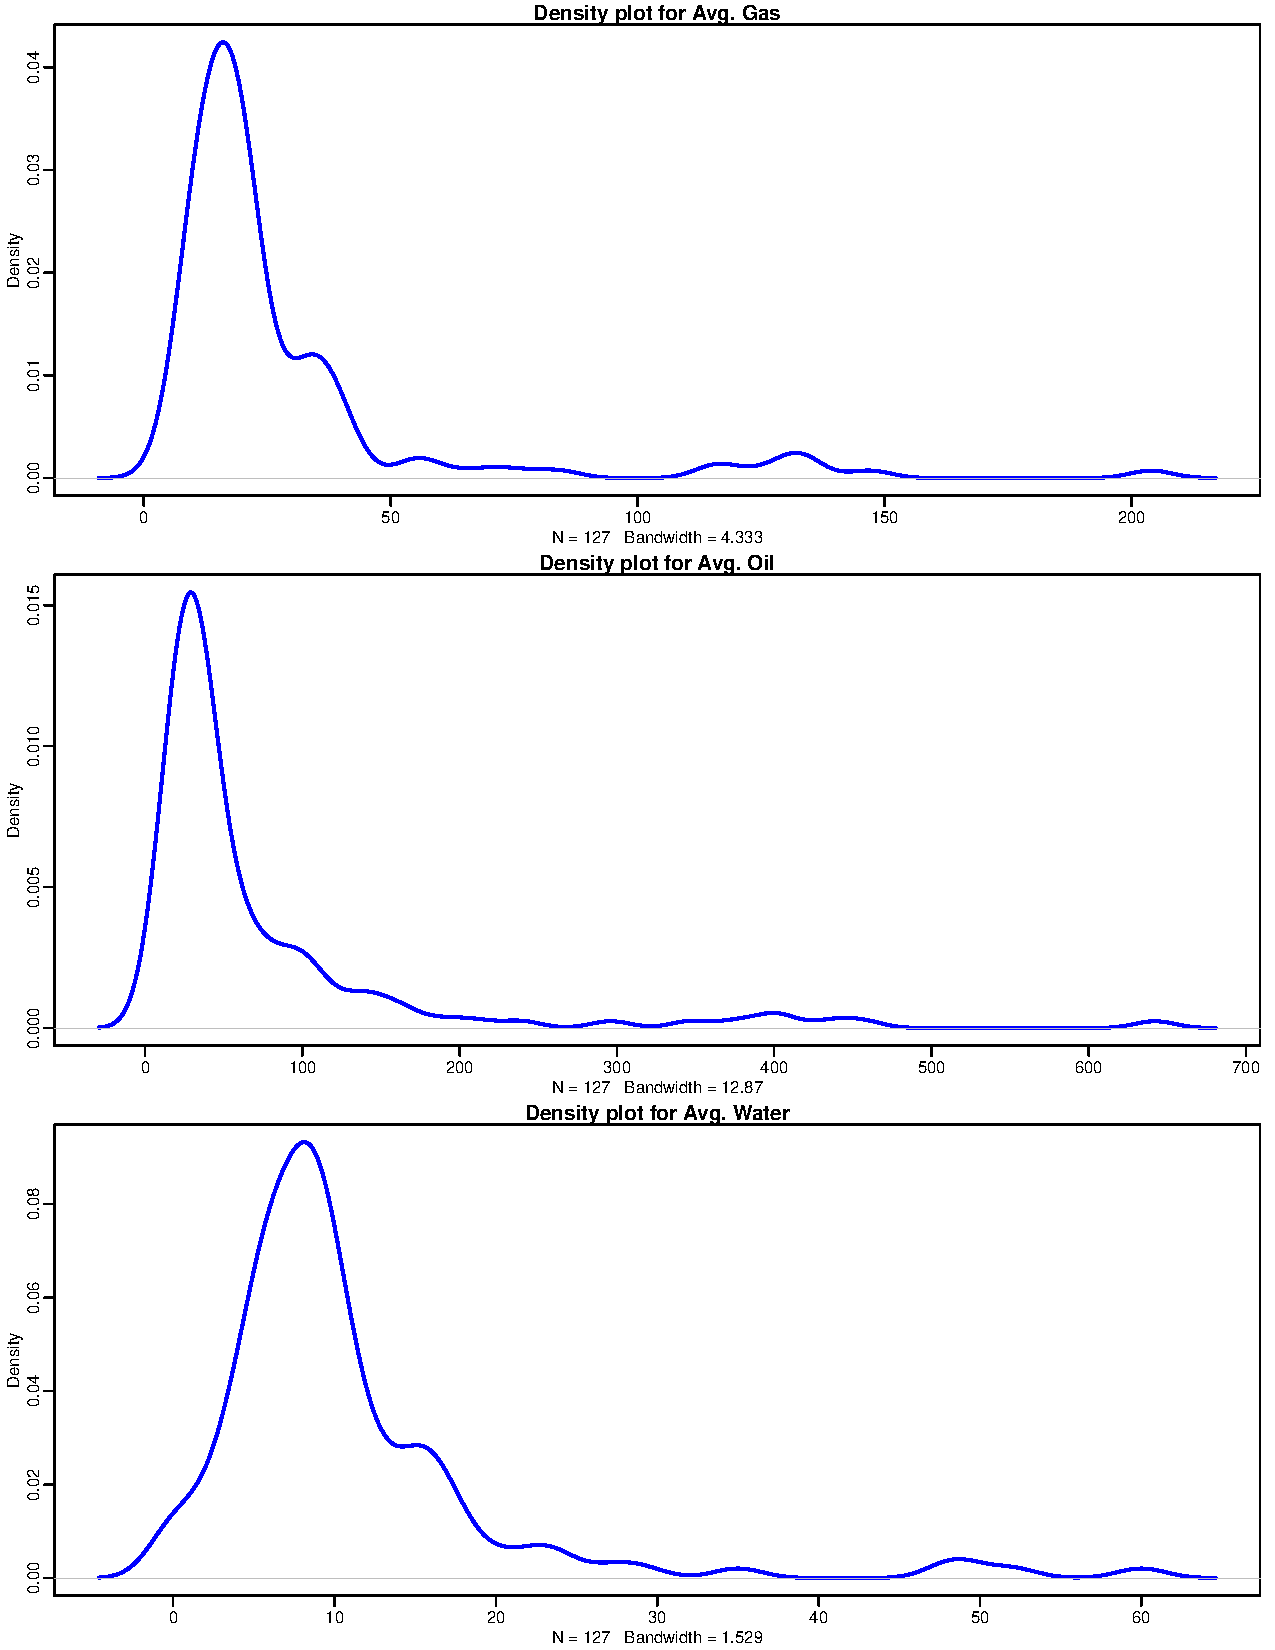
\includegraphics[width=0.9\textwidth]{DensityTS}
 	\caption{$$Density Plots of Avg. Gas , Oil and Water$$}
 	\label{fig1:DensityTS}
 \end{figure}

 \begin{figure}
	\centering
	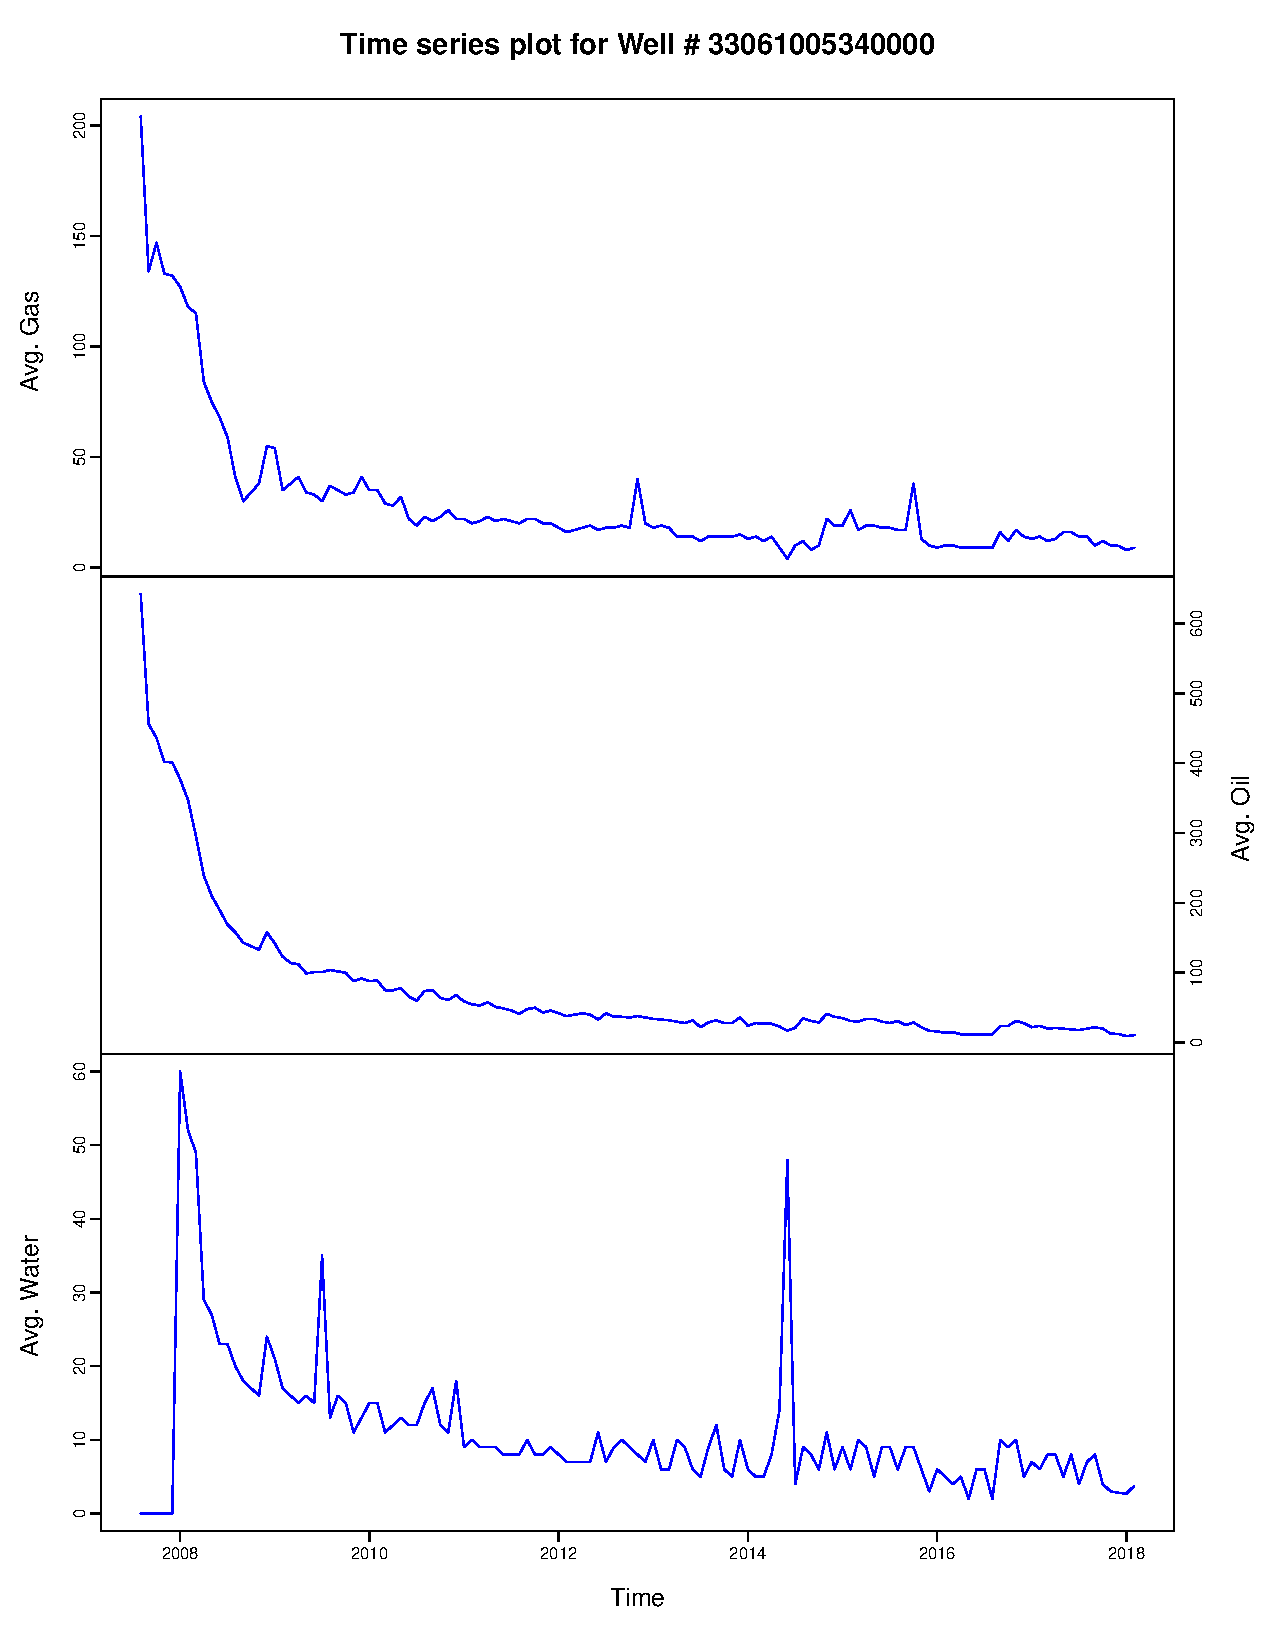
\includegraphics[width=0.9\textwidth]{TS}
	\caption{$$Time Series Plots of Avg. Gas , Oil and Water$$}
	\label{fig1:TS}
\end{figure}

\newpage

\section{Data Analysis}
\subsection{Model Formulation}

We consider two broad categories of model formulation for modelling the stochastic processes of Avg. Oil, Avg. Gas and Avg. Water. These are 

\begin{enumerate}
	\item  \textbf{Semi - parametric family of regression ~\cite{RJC2009}  ~\cite{Gam-R-mgcv} }\\
	
	Here at start, given that the function of the processes are non linear with respect to time as shown in Figure \ref{fig1:TS}, we will use Bspline Basis Functions with a modification suggested by Finbarr O’Sullivan of University
	College Cork, in Ireland called cubic O’Sullivan splines. The O-splines approximate the underlying regression functions
	as
	
	$$
	f(x) = \beta_{0} + \beta_{1}x + \sum_{1}^{K}u_kz_k(x)  \\	
	$$	
	
	where $x$ is time , $z_k(.)$ are the O - Sullivan Splines. $f(x)$ is linear if $u_1 = u_2 \dots = 0$.
	
	With a larger value of K and  appropriate penalization, $f(x)$ can approximate very complex shapes.
   
   \newpage
   
	
	\item  \textbf{ ARIMA based models }
	
	Standard model selection and estimation procedures as learnt under SARIMA modelling techniques , which is 
	
    \begin{center}
    		\textbf{$\Phi{_P}{(B^s)}\phi{_p}{(B)}{\nabla{_s}}^D{\nabla}^dx_t = \delta + \Theta{_Q}{(B^s)}\theta{(B)}w_t$}
    \end{center}
where 

$\Phi{_P}{(B^s)}$ and $ \phi{_p}{(B)}$ are seasonal and non-seasonal Auto-Regressive Operators of order P and p
 respectively.  \\
${\nabla{_s}}^D$  and$ {\nabla{}}^d$ are seasonal and non-seasonal difference operator respectively. \\
$\Theta{_Q}{(B^s)}$ and $\theta{(B)}$ are seasonal and non-seasonal Moving Average Operators of order Q and q
respectively.  

For model formulation we follow Exploratory Data Analysis techniques using difference to de-trend the series and plot ACF and PACF to get a set of plausible values of p, q, d, P, Q, D and S. 

Given that the density of the observations are highly non normal with high variance as shown in Figure \ref{fig1:DensityTS} and \ref{fig1:TS}, we transform the series to logarithmic scale to contain both of these. The transformed and differenced series is plotted in Figure \ref{fig1:densitylog} and \ref{fig1:DensityTS}. We notice non-normality in data and while, better transforms are
available to normalize and contain the variance we choose to stick to log transforms since we can easily back transform the forecasts to original scale along with standard errors. 

We look individually at ACF and PACF plots for the three processes to get plausibal set of values of the orders of the model.


\begin{enumerate}
	\item \textbf{Avg. Gas}\\
	Figure \ref{fig1:acf2_gas} shows involvement of seasonal components at lag 1 and 2. We note that its almost non significant at $$\alpha = 0.05 $$. We also see presence of effects of AR and MA non-seasonal components. Thus the plausible set of values of the orders for which we estimate and diagnose the model are for 
	S = 12 , 0 , Q = 2 , 0 , P = 0 , D = 0 , d = 1 , q = 1 ,4 , p = 2. 
	
	\item \textbf{Avg. Oil}\\
	Figure \ref{fig1:acf2_oil} does not show any interesting affects of correlation.  We notice weakly significant $$\hat\rho{(11)}$$ so we diagnose and estimate the model with both q = 0 and 11, d=1.
	
	\item \textbf{Avg. Water}\\
	Figure \ref{fig1:acf2_Water} shows involvement of non-seasonal components only. Thus the plausible set of values of the orders for which we estimate and diagnose the model are for 
	S=0 , P = Q = 0 , p = 1 , 2 , q = 1 , d = 1. 
\end{enumerate}
  


\end{enumerate}

\begin{figure}
	\centering
	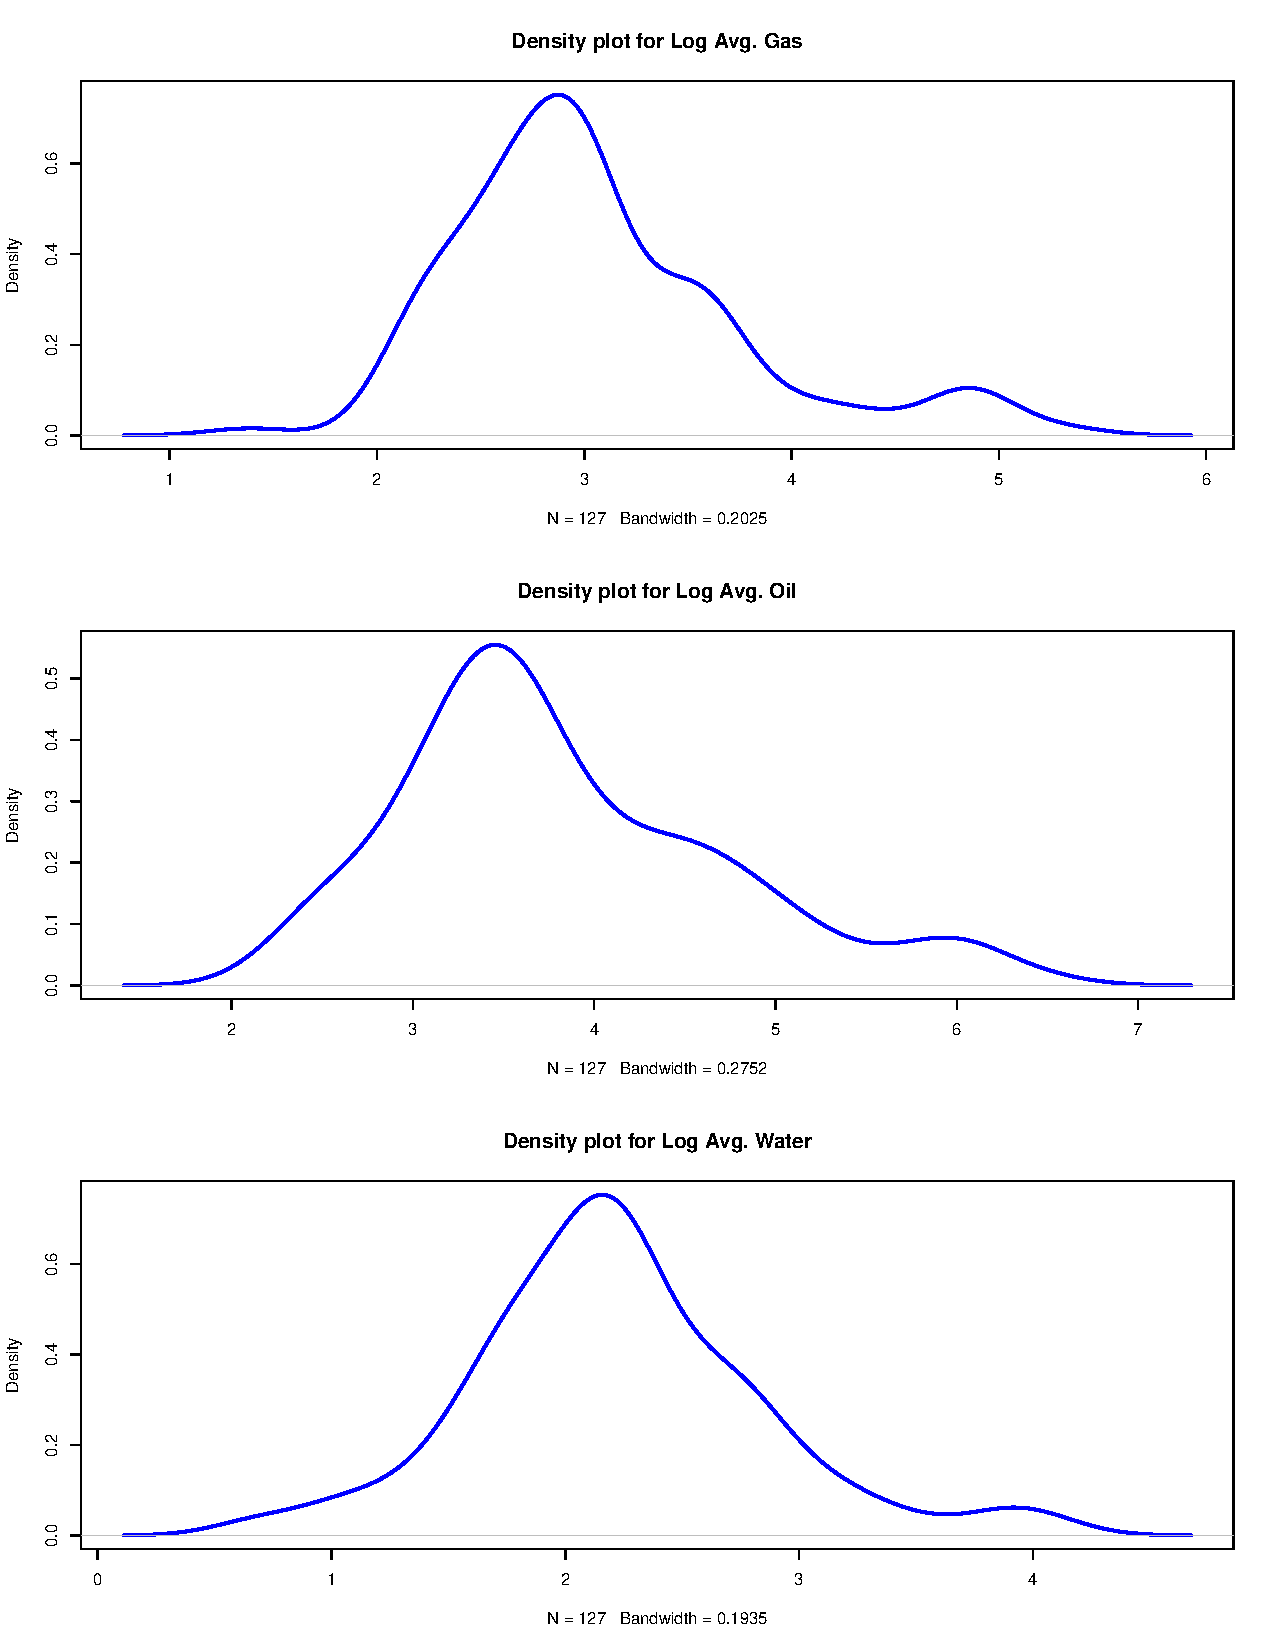
\includegraphics[width=0.6\textwidth]{densitylog}
	\caption{$$Density of the Time Series after Log$$}
	\label{fig1:densitylog}
\end{figure}
\begin{figure}
	\centering
	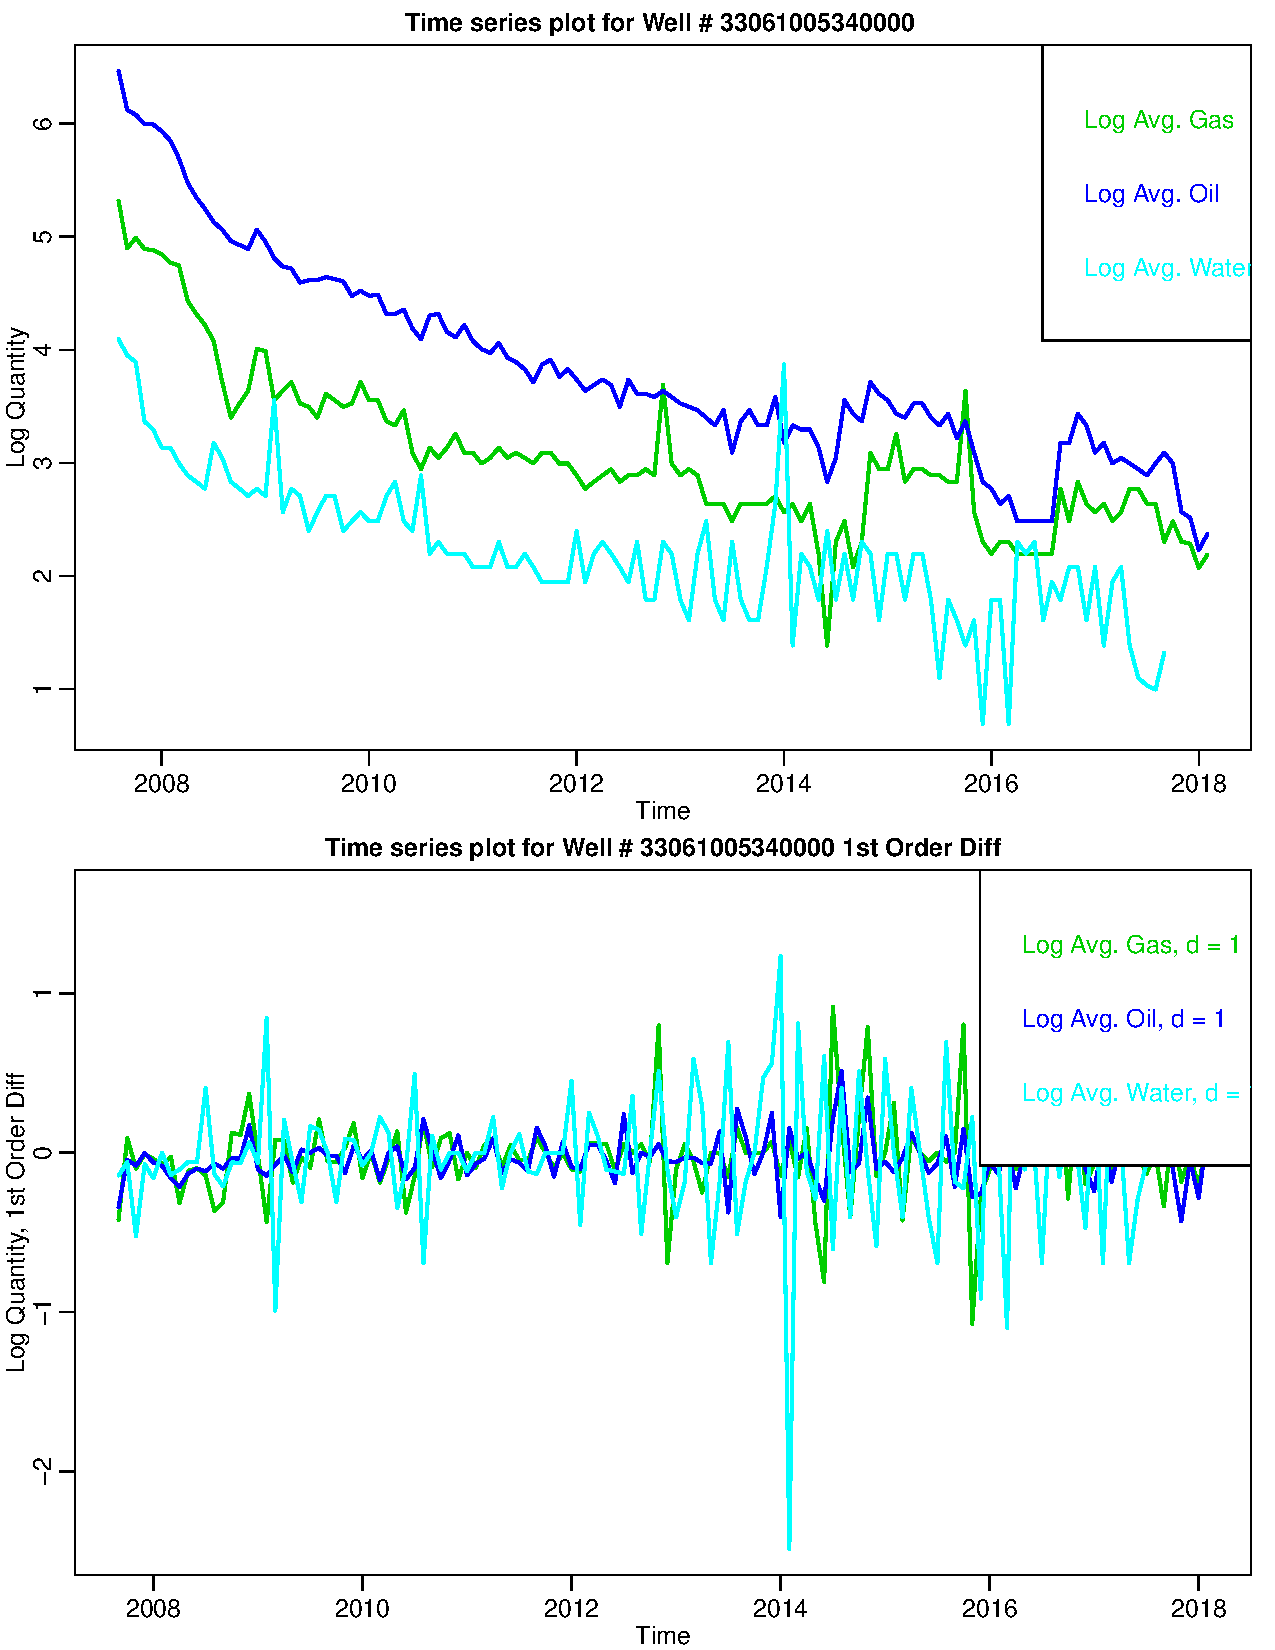
\includegraphics[width=0.6\textwidth]{TSLoganddiff}
	\caption{$$Time Series after transformation and Difference$$}
	\label{fig1:TSLoganddiff}
\end{figure}
\begin{figure}
	\centering
	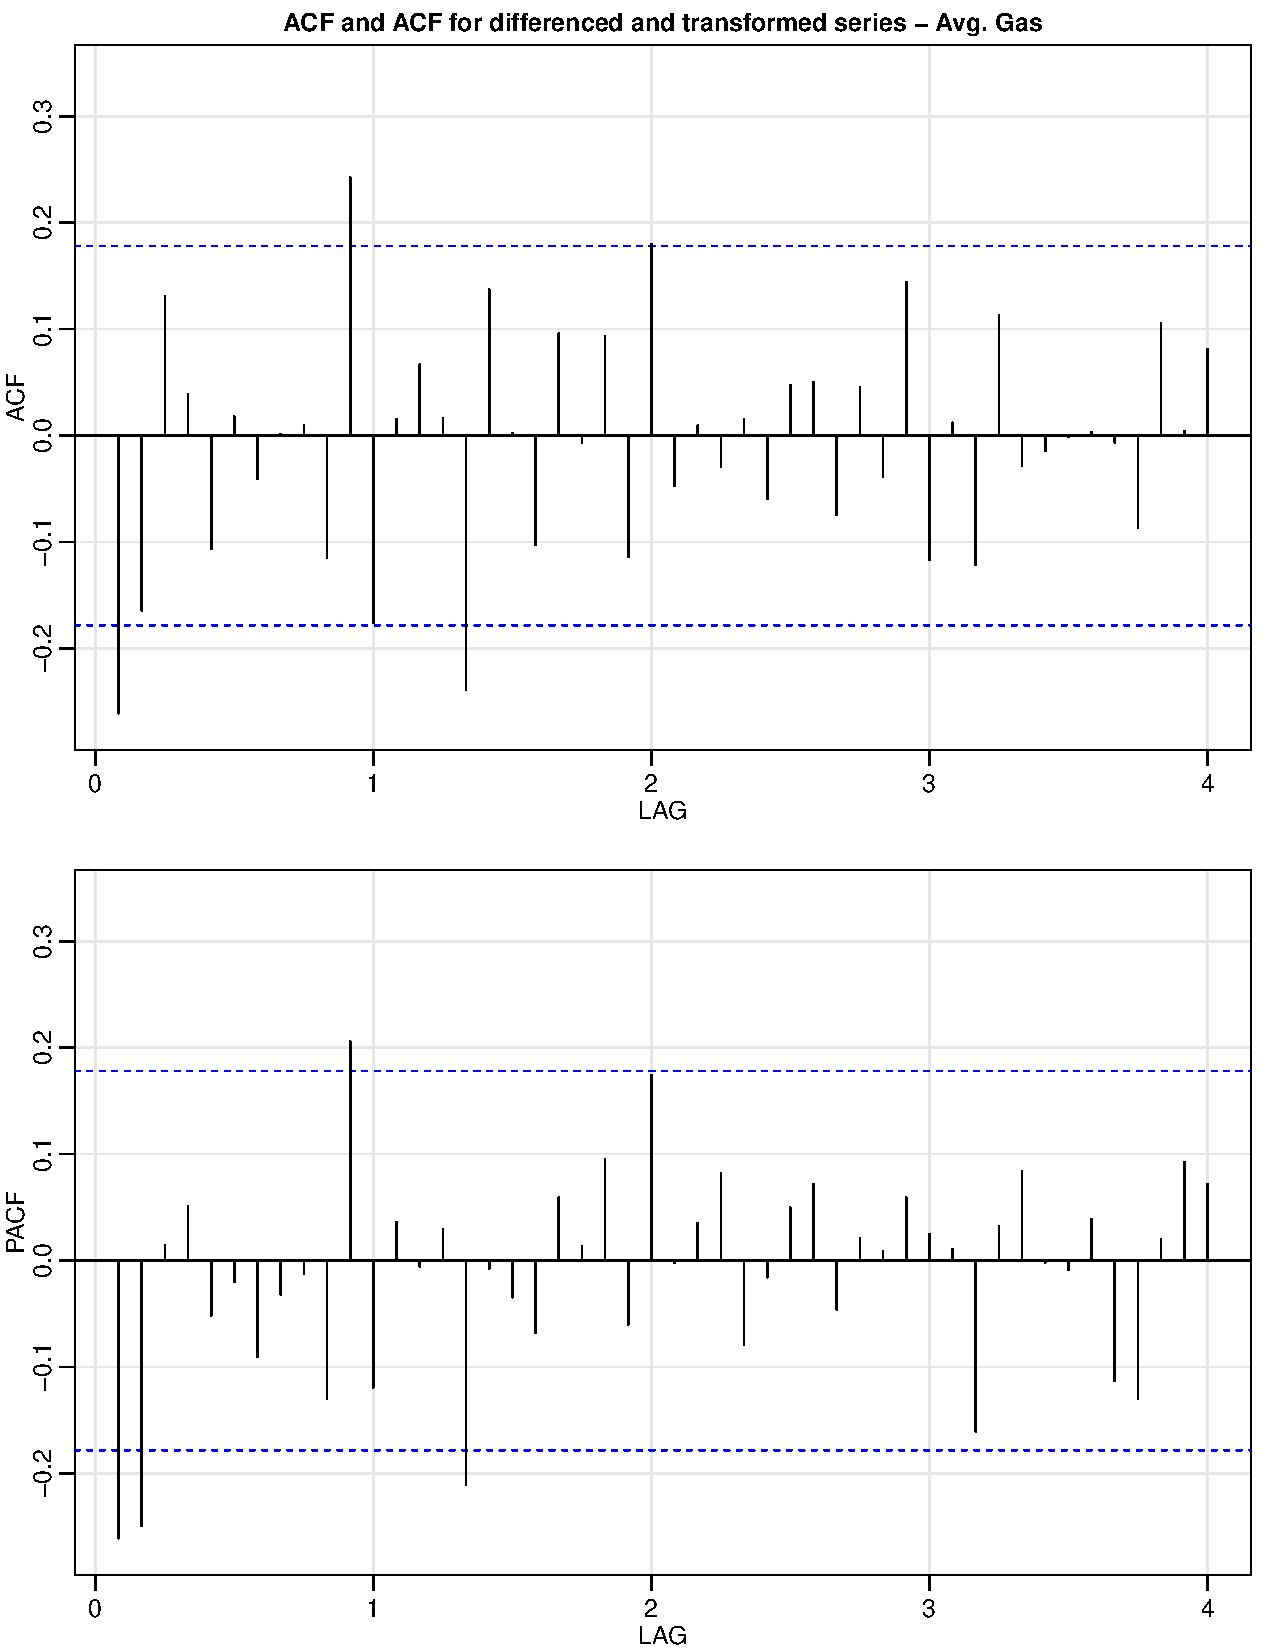
\includegraphics[width=0.6\textwidth]{acf2_gas}
	\caption{$$ACF and PACF plot for Avg. Gas$$}
	\label{fig1:acf2_gas}
\end{figure}
\begin{figure}
	\centering
	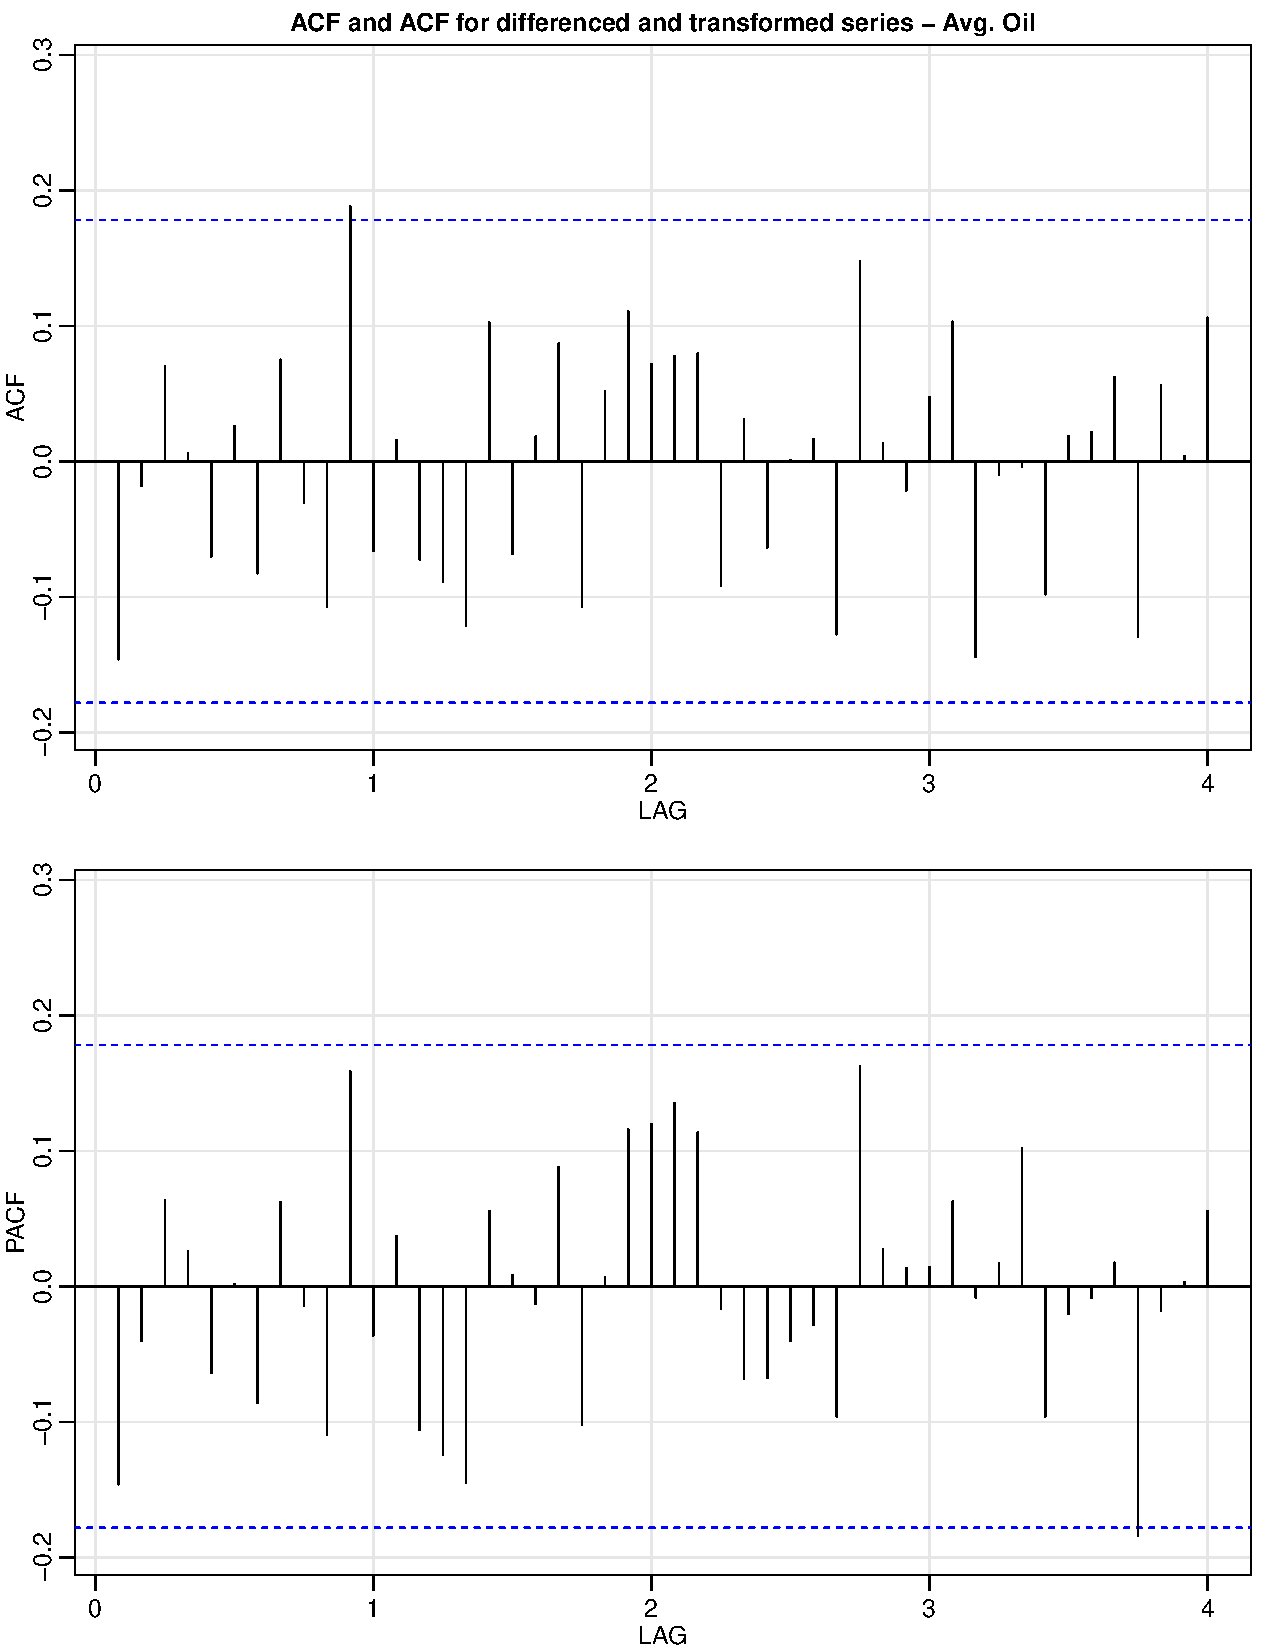
\includegraphics[width=0.6\textwidth]{acf2_oil}
	\caption{$$ACF and PACF plot for Avg. Oil$$}
	\label{fig1:acf2_oil}
\end{figure}
\begin{figure}
	\centering
	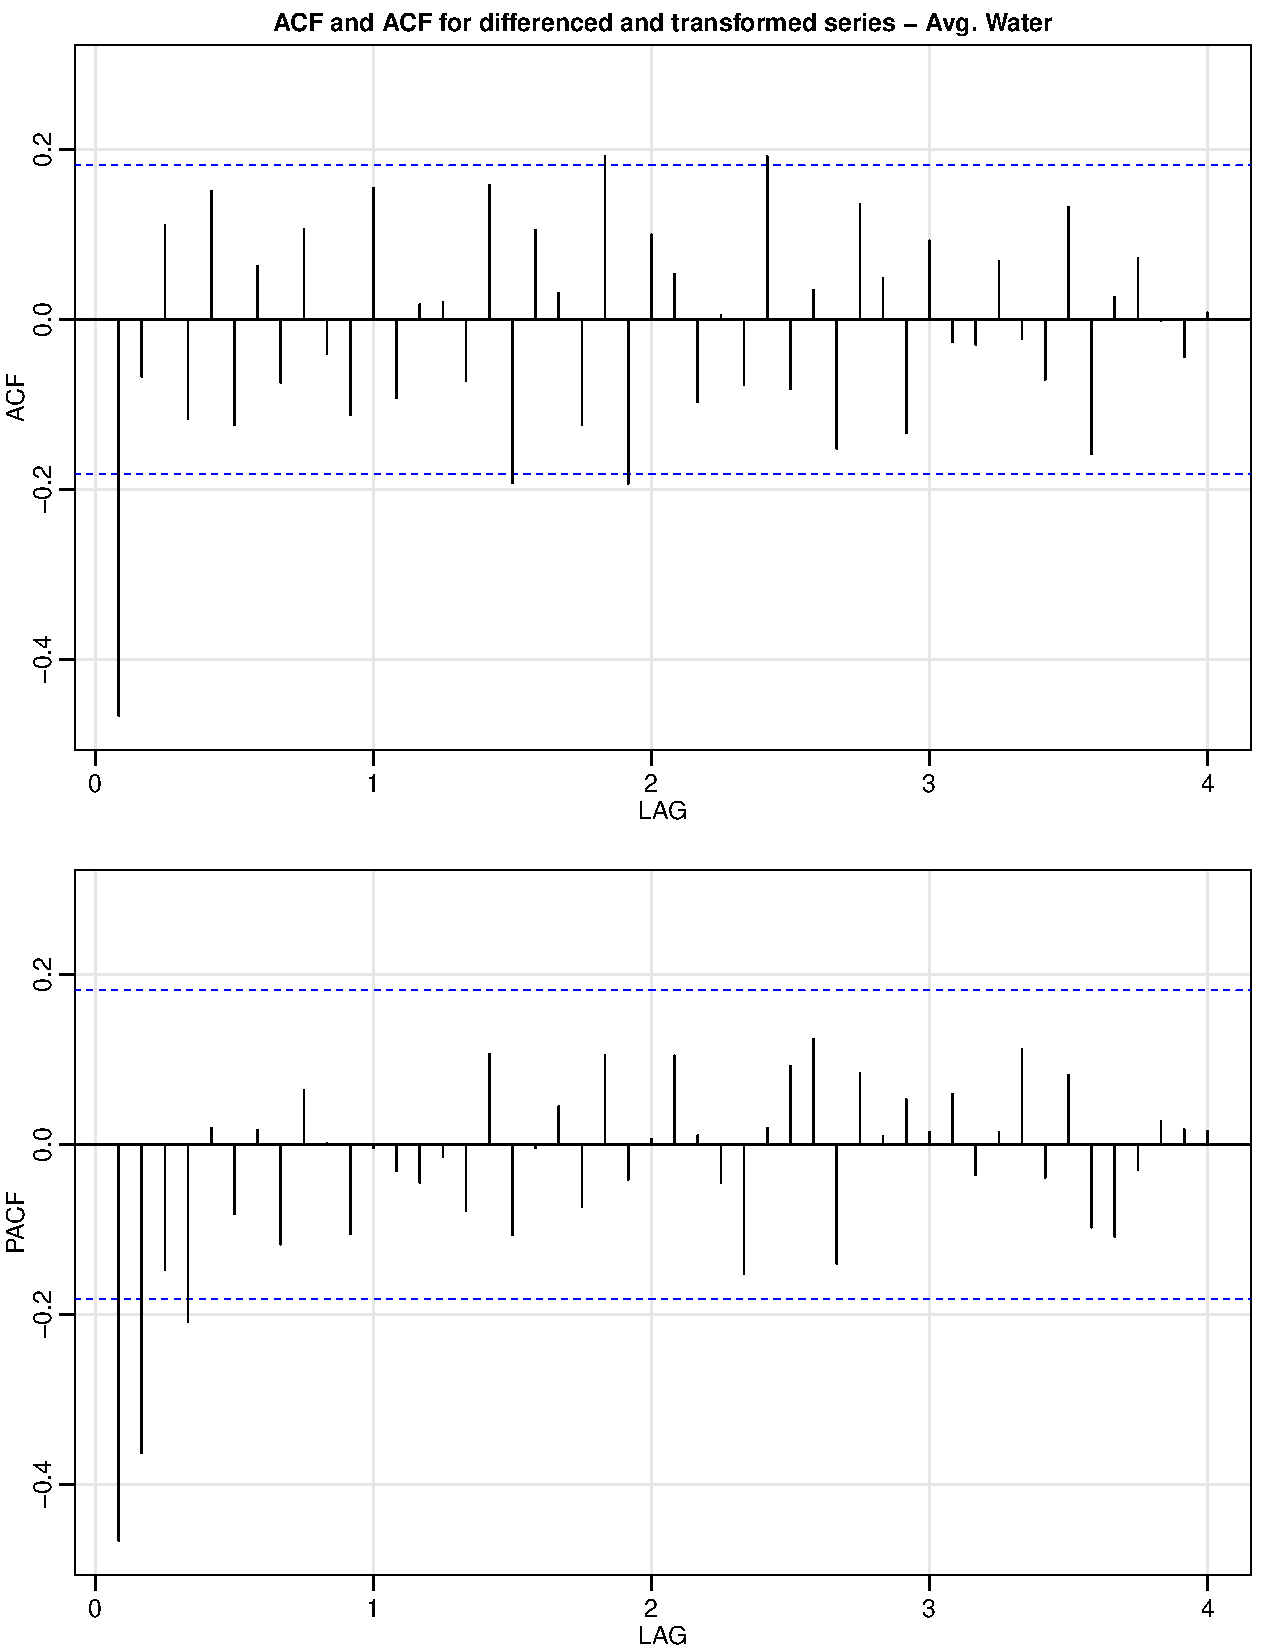
\includegraphics[width=0.6\textwidth]{acf2_Water}
	\caption{$$ACF and PACF plot for Avg. Water$$}
	\label{fig1:acf2_Water}
\end{figure}

\newpage
\subsection{Model Estimation}
\begin{enumerate}
	\item  \textbf{Semi - parametric family of regression ~\cite{RJC2009}  ~\cite{Gam-R-mgcv} }\\
 We look at modeling the data via package \verb|mgcv|~\cite{Gam-R-mgcv}. The mathematical details, derivations and estimations are given referenced in ~\cite{RJC2009} , ~\cite{REML-Mgcv} and ~\cite{Gam-Smoothing-Woods}

A semi-parametric model was thus fit to a particular well number 33061005340000 and estimates were obtained for all the three processes. The model summaries are as below.

\begin{enumerate}
\item Avg. Gas : Figure \ref{fig1:GasGam} shows the model formulation and estimation of parameters via R . We see a significant effect of time as we anticipate. \\
\item Avg. Oil : Figure \ref{fig1:OilGam} shows the model formulation and estimation of parameters via R . We see a significant effect of time as we would anticipate. \\
\item Avg. Water : Figure \ref{fig1:WaterGam} shows the model formulation and estimation of parameters via R . We see a significant effect of time as we would anticipate. 
\end{enumerate}

Note that in all of the above fits we have chosen the number of basis functions to be used as 30. This  was arrived at after running few diagnostic procedures during the model formulation. Since the number was very high, so was the number of estimated parameters. The estimated values of these are thus not shown in this document 

 The fitted values for all of the above fits are plotted in Figure \ref{fig1:GAMFitsUntransformed}. We notice that the fitted values follow closely the observations in all the three processes. There are, however, observations where fits perform poorly and may be contributing to the large value of cross validation error as reported by \verb|mgcv|. This occurs specially for Water dataset. We also notice observations that does not follow the usual pattern in the data set. 


\begin{figure}
	\centering
	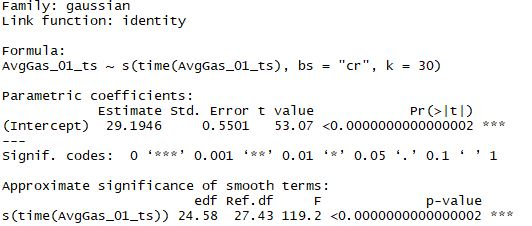
\includegraphics[width=0.6\textwidth]{GasGam}
	\caption{$$Semi-par regression of Avg. Gas with Time$$}
	\label{fig1:GasGam}
\end{figure}

\begin{figure}
	\centering
	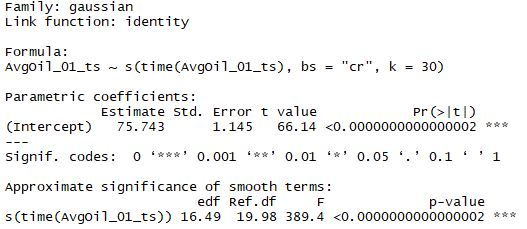
\includegraphics[width=0.6\textwidth]{OilGam}
	\caption{$$Semi-par regression of Avg. Oil with Time$$}
	\label{fig1:OilGam}
\end{figure}   

\begin{figure}
	\centering
	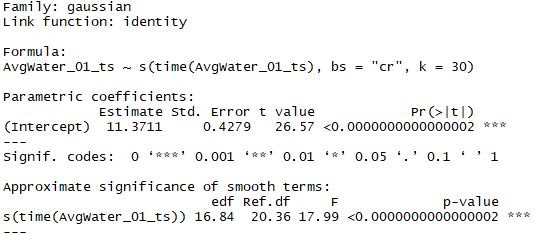
\includegraphics[width=0.6\textwidth]{WaterGam}
	\caption{$$Semi-par regression of Avg. Water with Time$$}
	\label{fig1:WaterGam}
\end{figure}	


\begin{figure}
	\centering
	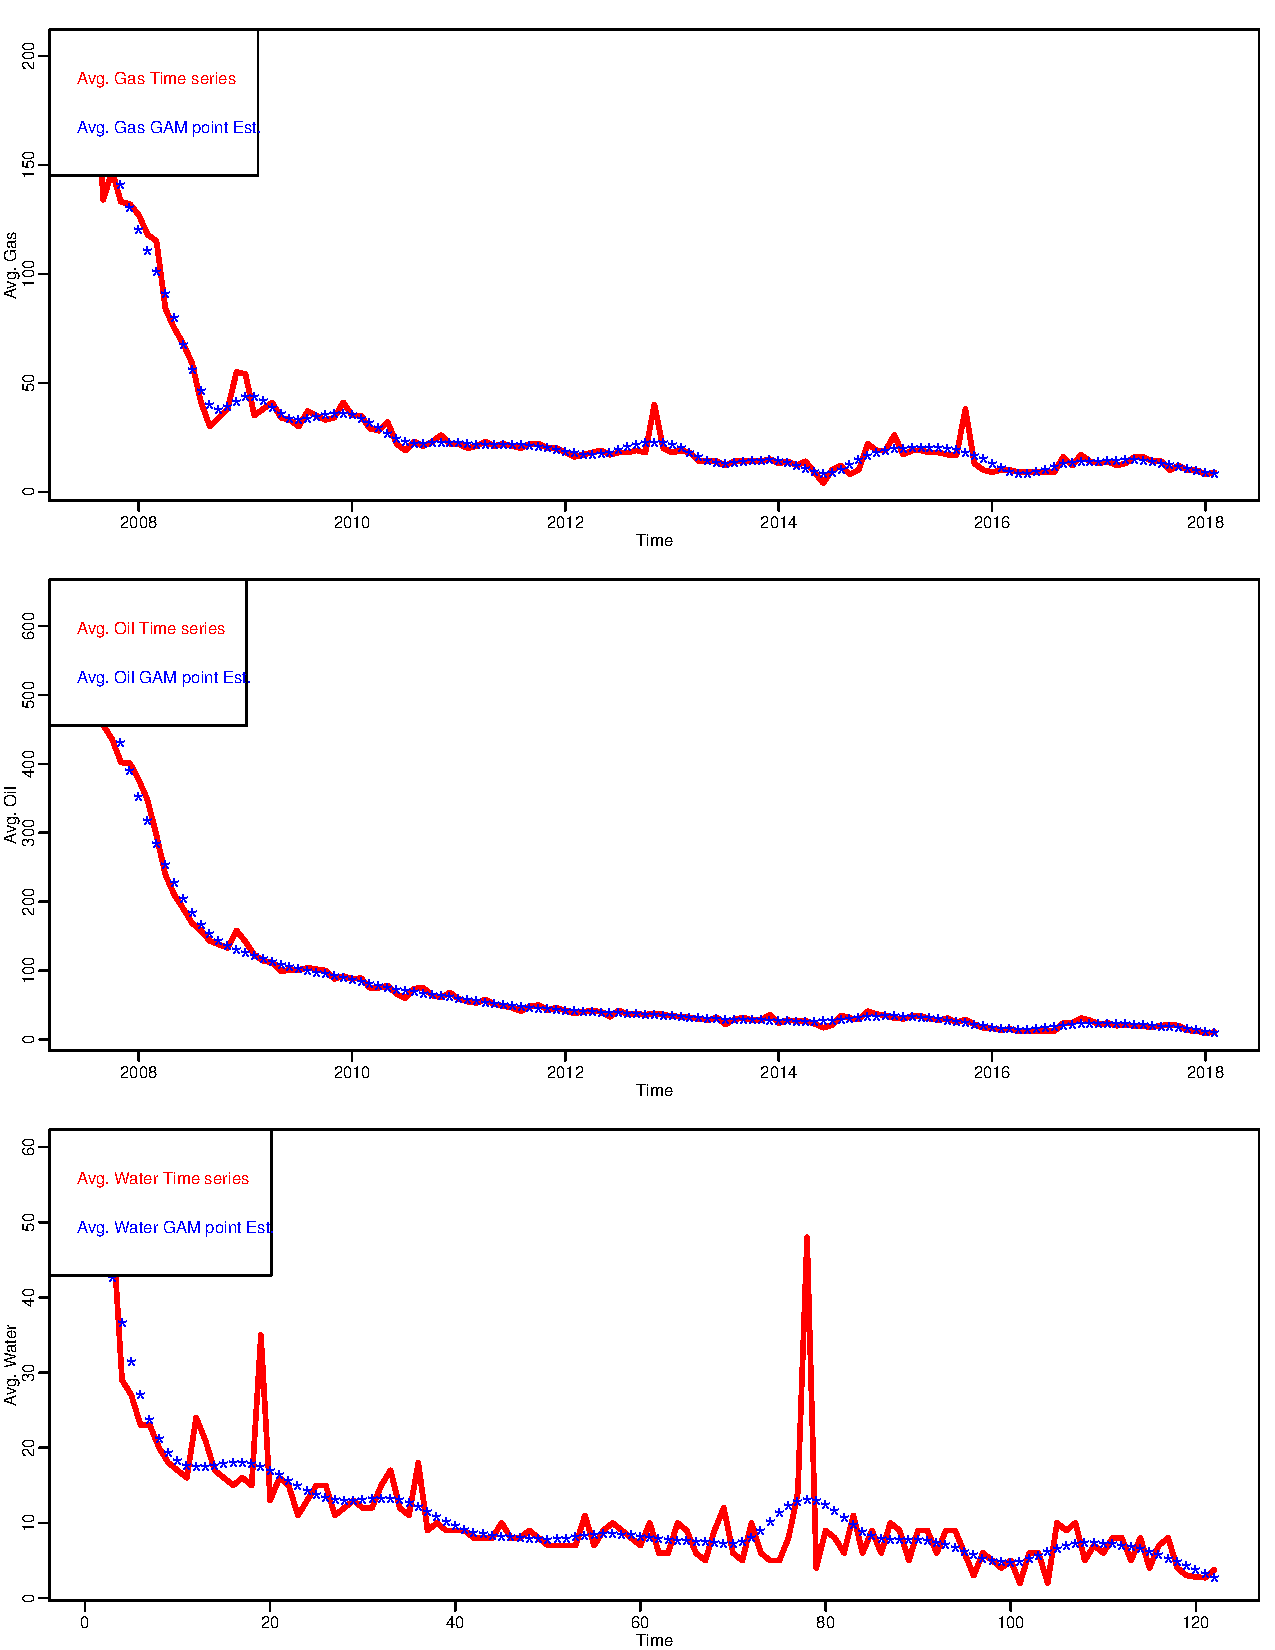
\includegraphics[width=0.6\textwidth]{GAMFitsUntransformed}
	\caption{$$Fiited vs Observed via GAM model$$}
	\label{fig1:GAMFitsUntransformed}
\end{figure}


\newpage
	\item  \textbf{ ARIMA based models }

We estimate the parameters of the model using \verb|astsa| package in \verb|R|. 

For Avg. Gas process we settle with a simpler model with q = 1 and d = 1 and rest all 0 based on lowest value of AIC, BIC and AICc. For brevity, the model estimated parameters is omitted in this document. We proceed with this model for forecast Avg. Gas but we caution that a more robust procedure multi- fold cross validation might be necessary to further validate the model. 

For Avg. Oil process we settle with a simpler model with q = 1 and d = 1 and rest all 0 based on lowest value of AIC, BIC and AICc. For brevity, the model estimated parameters is omitted in this document. We proceed with this model for forecast Avg. Gas but we caution that a more robust procedure multi- fold cross validation might be necessary to further validate the model. 

For Avg. Water process we settle with a simpler model with q = 1 and d = 1 and rest all 0 based on lowest value of AIC, BIC and AICc. For brevity, the model estimated parameters is omitted in this document. We proceed with this model for forecast Avg. Gas but we caution that a more robust procedure multi- fold cross validation might be necessary to further validate the model. 


\end{enumerate}

\newpage
\subsection{Model Diagnostics}
\begin{enumerate}
	\item  \textbf{Semi - parametric family of regression ~\cite{RJC2009}  ~\cite{Gam-R-mgcv} }\\

The residuals from the fits in the Model \ref{fig1:GasGam} , \ref{fig1:OilGam} and \ref{fig1:WaterGam} were extracted and plotted 
with respect to time to find any visual evidence of patterns in the residuals. Their ACF plots was also obtained to provide support to the assumptions of randomness in the residuals. Both these plots are shown in the Figure \ref{fig1:ResidualsGAMUntransformed_Diag} . The plots are for all the three fits. We notice that plots indicate a significant autocorrelation of the order 3 in Avg. Oil model indicating a need for modeling serially correlated errors as well. We will analyze this again in ARIMA model to confirm if we have a better model. We also notice the presence of influential points in all the three timeseries further indicating that we may need to understand the behavior of the processes around these points. At the moment we will ignore and accept these anomalies in the dataset with the caveat that we may be missing to account for the scenario
when these anomalies occur.

\verb|Ljung-Box| test for whiteness in the residuals at values of lag 30 , 50 and 100 provide evidence, at critical value of $\alpha = 0.05$ , to support a fairly good fit to whiteness.However, we note that test of whiteness fails at lag of order 10 for Avg. Oil process when modeled with this approach. Plot \ref{fig1:Ljung-Box} shows the p-values obtained at various lags. 


	\begin{figure}
		\centering
		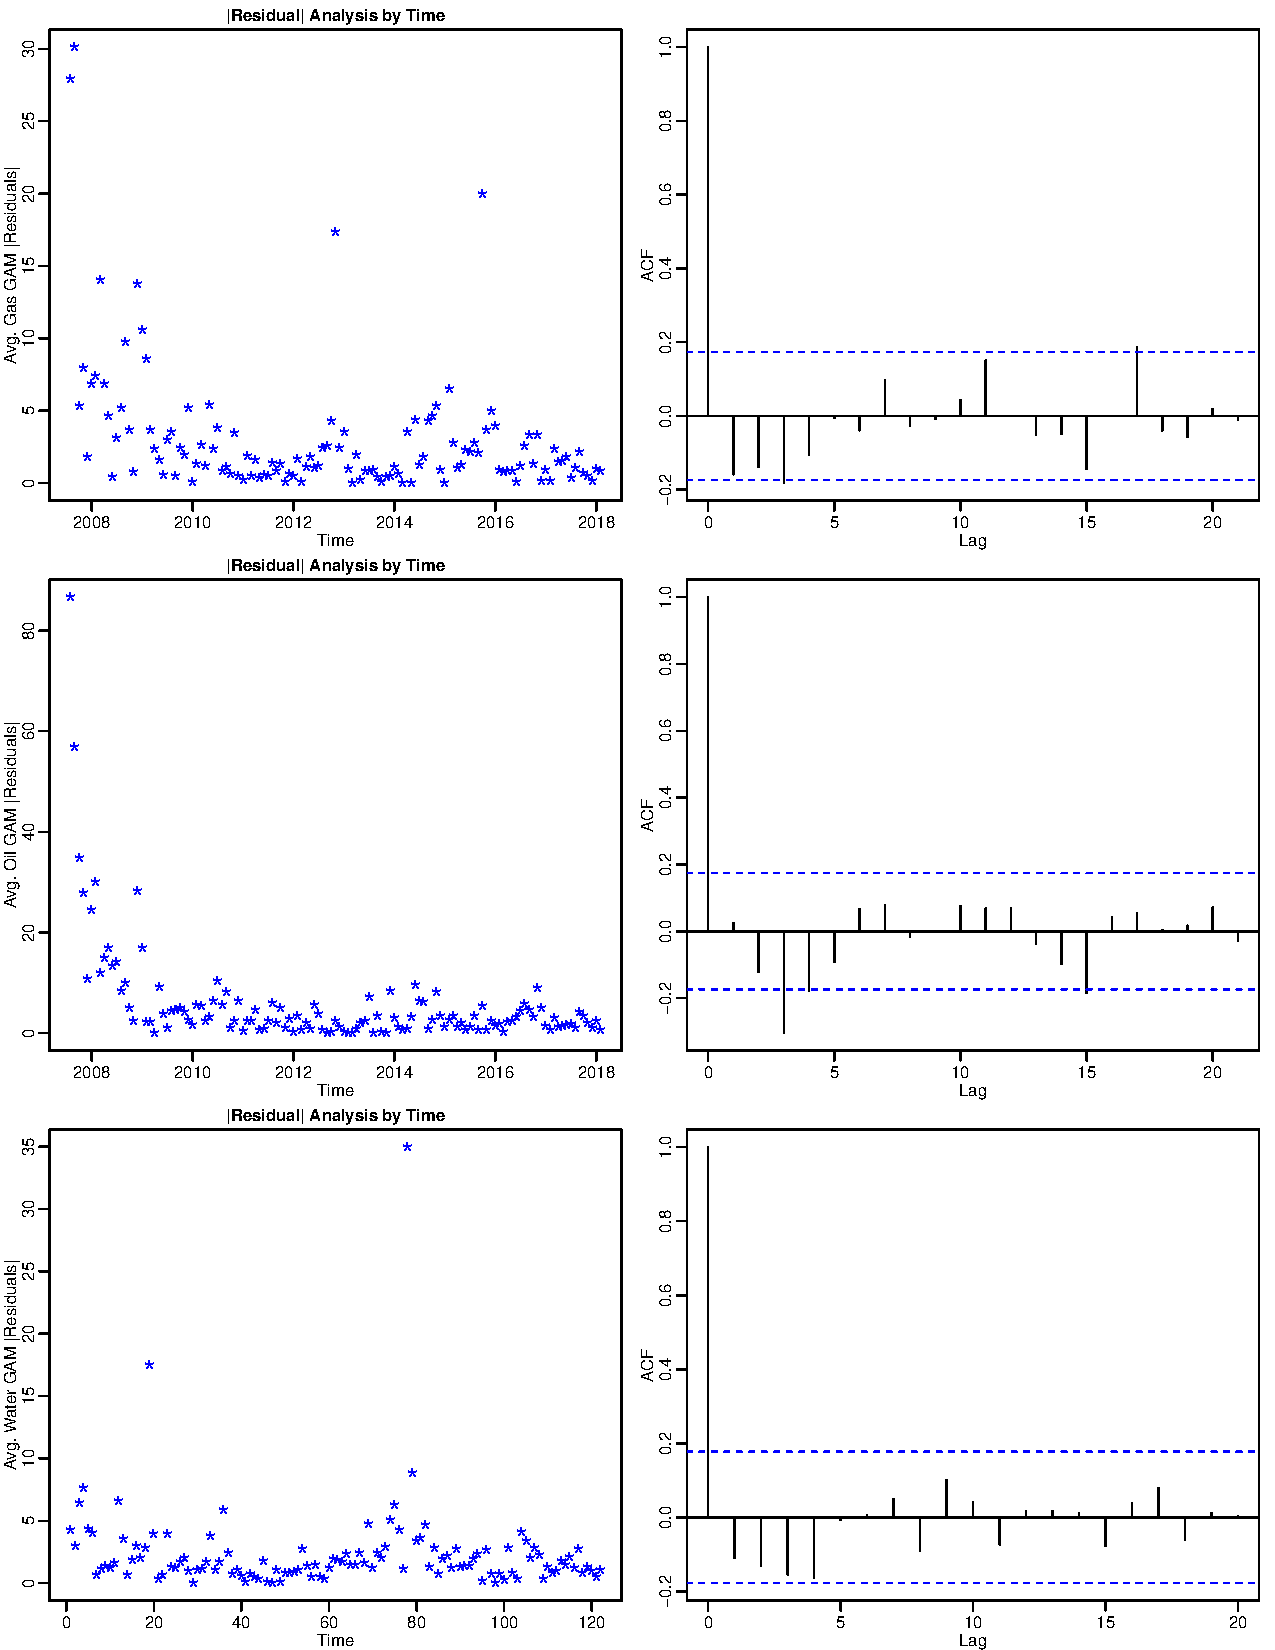
\includegraphics[width=0.6\textwidth]{ResidualsGAMUntransformed_Diag}
		\caption{$$|Residuals| in all the three fits$$}
		\label{fig1:ResidualsGAMUntransformed_Diag}
	\end{figure}
	\begin{figure}
	\centering
	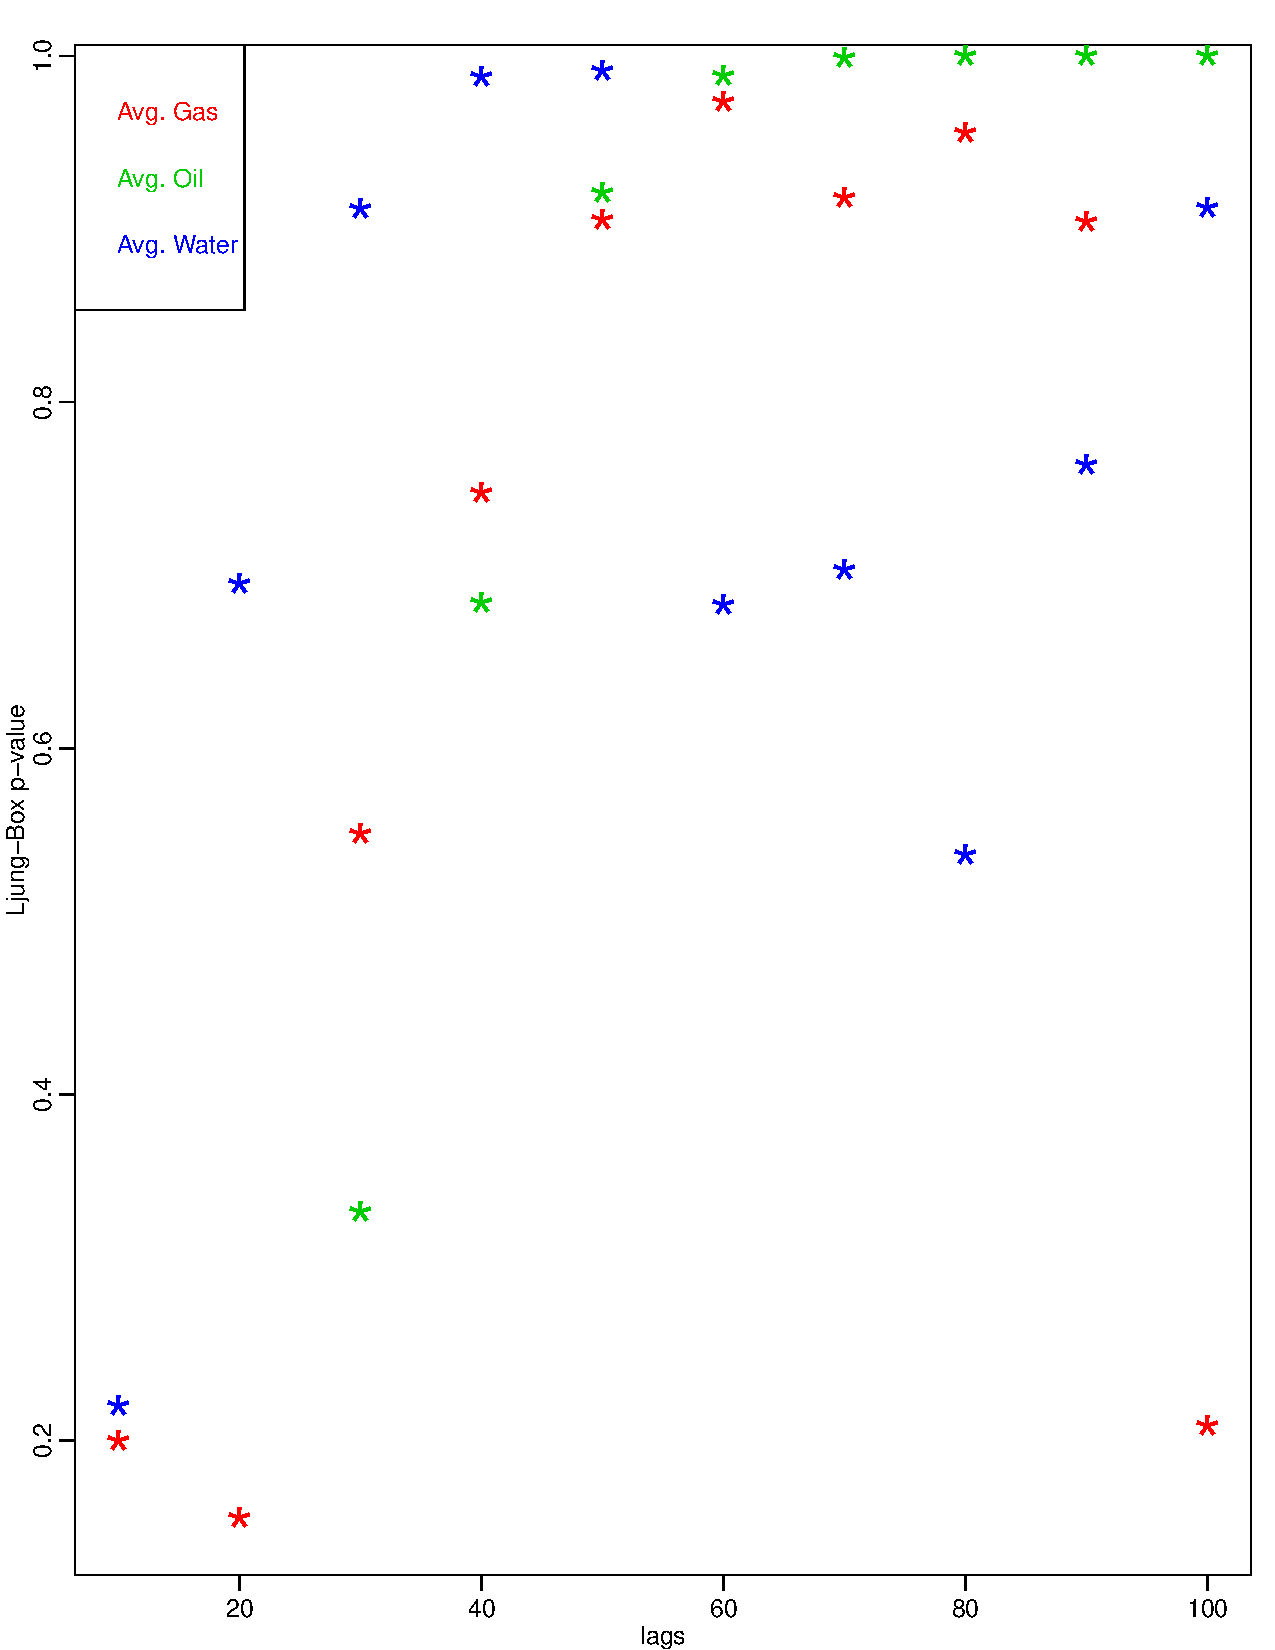
\includegraphics[width=0.6\textwidth]{Ljung-Box}
	\caption{Ljung-Box test p.value for the three series,$ \alpha = 0.05 $}
	\label{fig1:Ljung-Box}
\end{figure}
	
\newpage
\item  \textbf{ ARIMA based models }

We individually take a look at model diagnostics of the three processes of interest. 

\begin{enumerate}
	\item \textbf{Avg. Gas} \\
	
	Figure \ref{fig1:Sarima_Gas_Final} shows various plots detailing the analysis of the time series AVg. Gas. The test of Whiteness for the model looks positive indicating a good fit to the white noise. Normality in residuals is questionable and hence prediction intervals obtained from the point estimates of the forecasts might not be reliable. We will have to address this issue before we can forecast using this model. We also notice some significant auto correlation  in residuals which we will have to address. We think that having some explaining variables accounting information on anomalies will help us to address this issue. 
	
	Overall, while the fit of the model looks great the normality assumptions of the residuals does not look encouraging. 
	
	\item \textbf{Avg. Oil} \\
	
	Figure \ref{fig1:Sarima_Oil_Final} displays the check on residuals of the fitted values by the ARIMA model. We notice that we have great fit to white noise from the \verb|Ljung-Box| test. The normality assumptions on the residuals is acceptable and hence indicating a good and simple potential model.  
	
	\item \textbf{Avg. Water} \\
	
		Figure \ref{fig1:Sarima_Water_Final} displays the check on residuals of the fitted values by the ARIMA model. We notice that we have great fit to white noise from the \verb|Ljung-Box| test. The normality assumptions on the residuals is acceptable and hence indicating a good and simple potential model. 
		
\end{enumerate}


	\begin{figure}
	\centering
	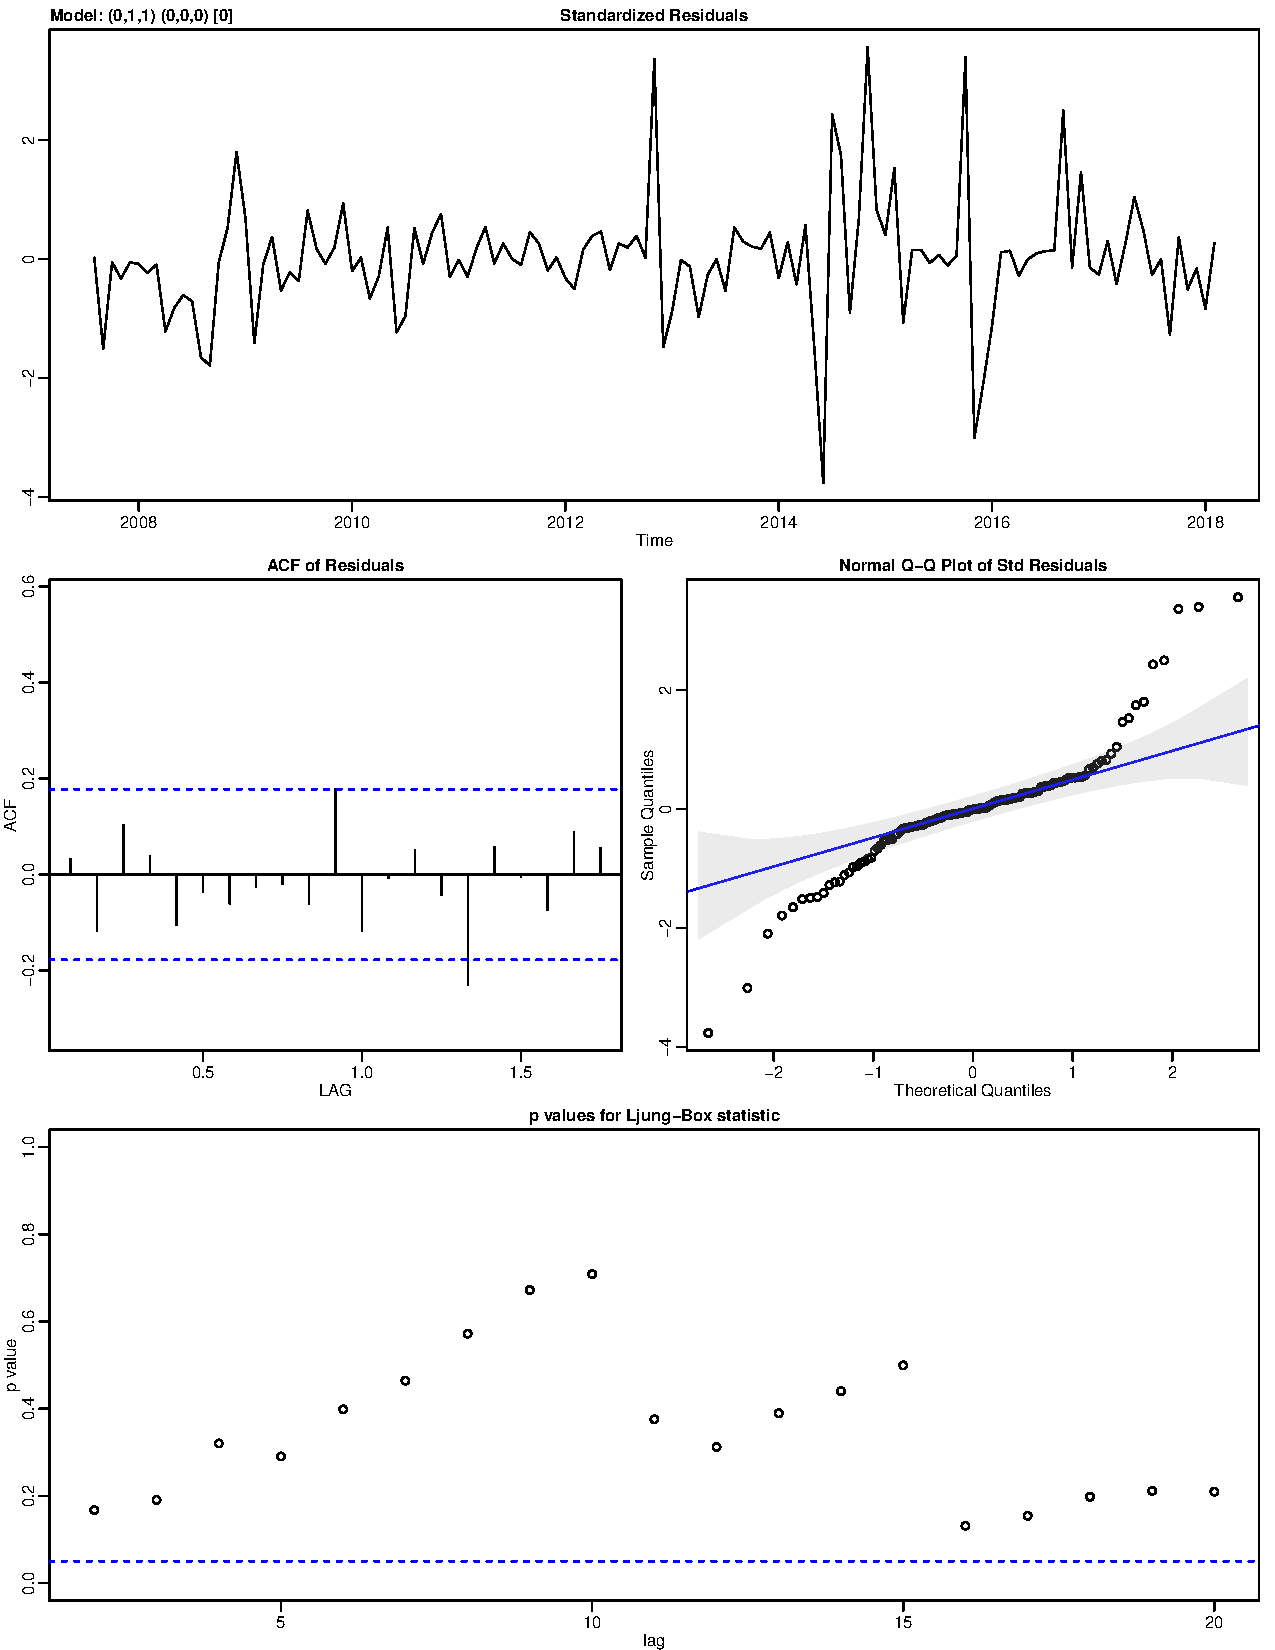
\includegraphics[width=0.6\textwidth]{Sarima_Gas_Final}
	\caption{Model Diagnostics , Avg. Gas}
	\label{fig1:Sarima_Gas_Final}
\end{figure}

	\begin{figure}
	\centering
	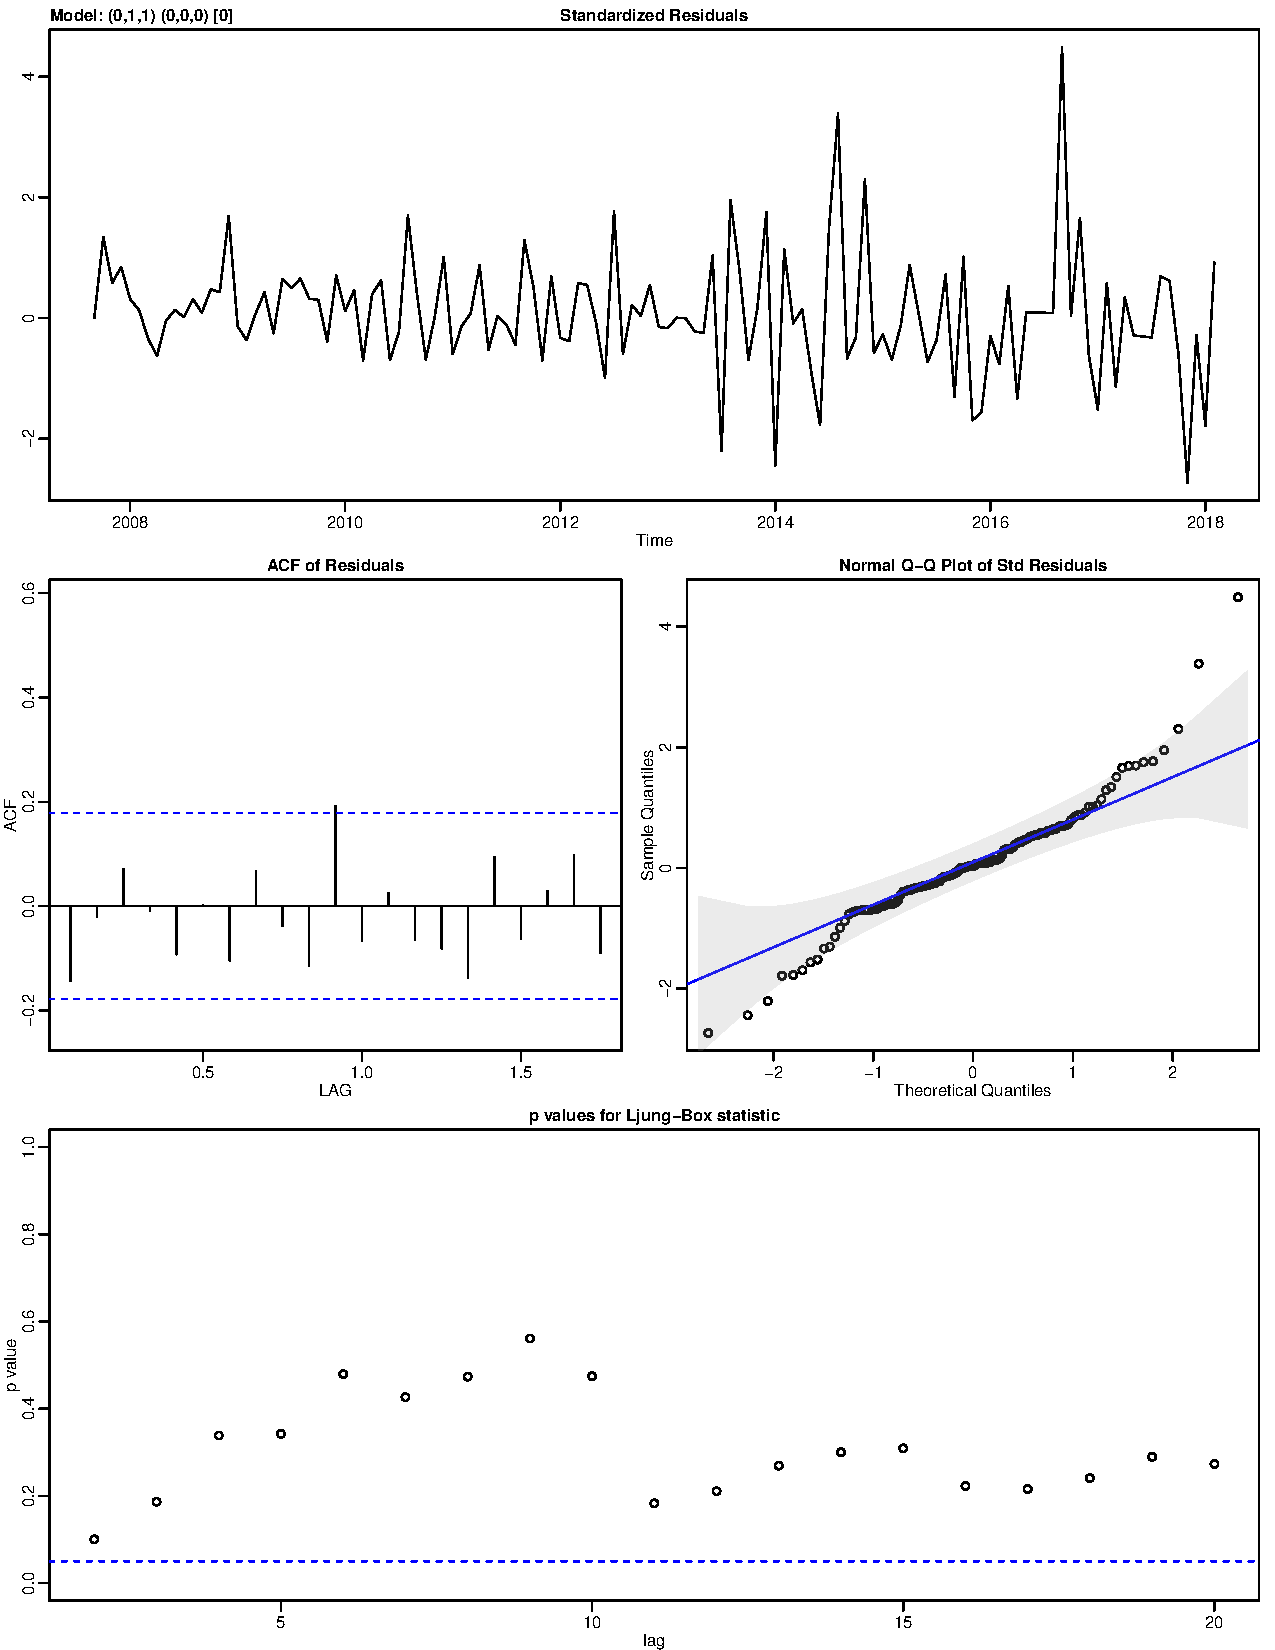
\includegraphics[width=0.6\textwidth]{Sarima_Oil_Final}
	\caption{Model Diagnostics , Avg. Oil}
	\label{fig1:Sarima_Oil_Final}
\end{figure}

	\begin{figure}
	\centering
	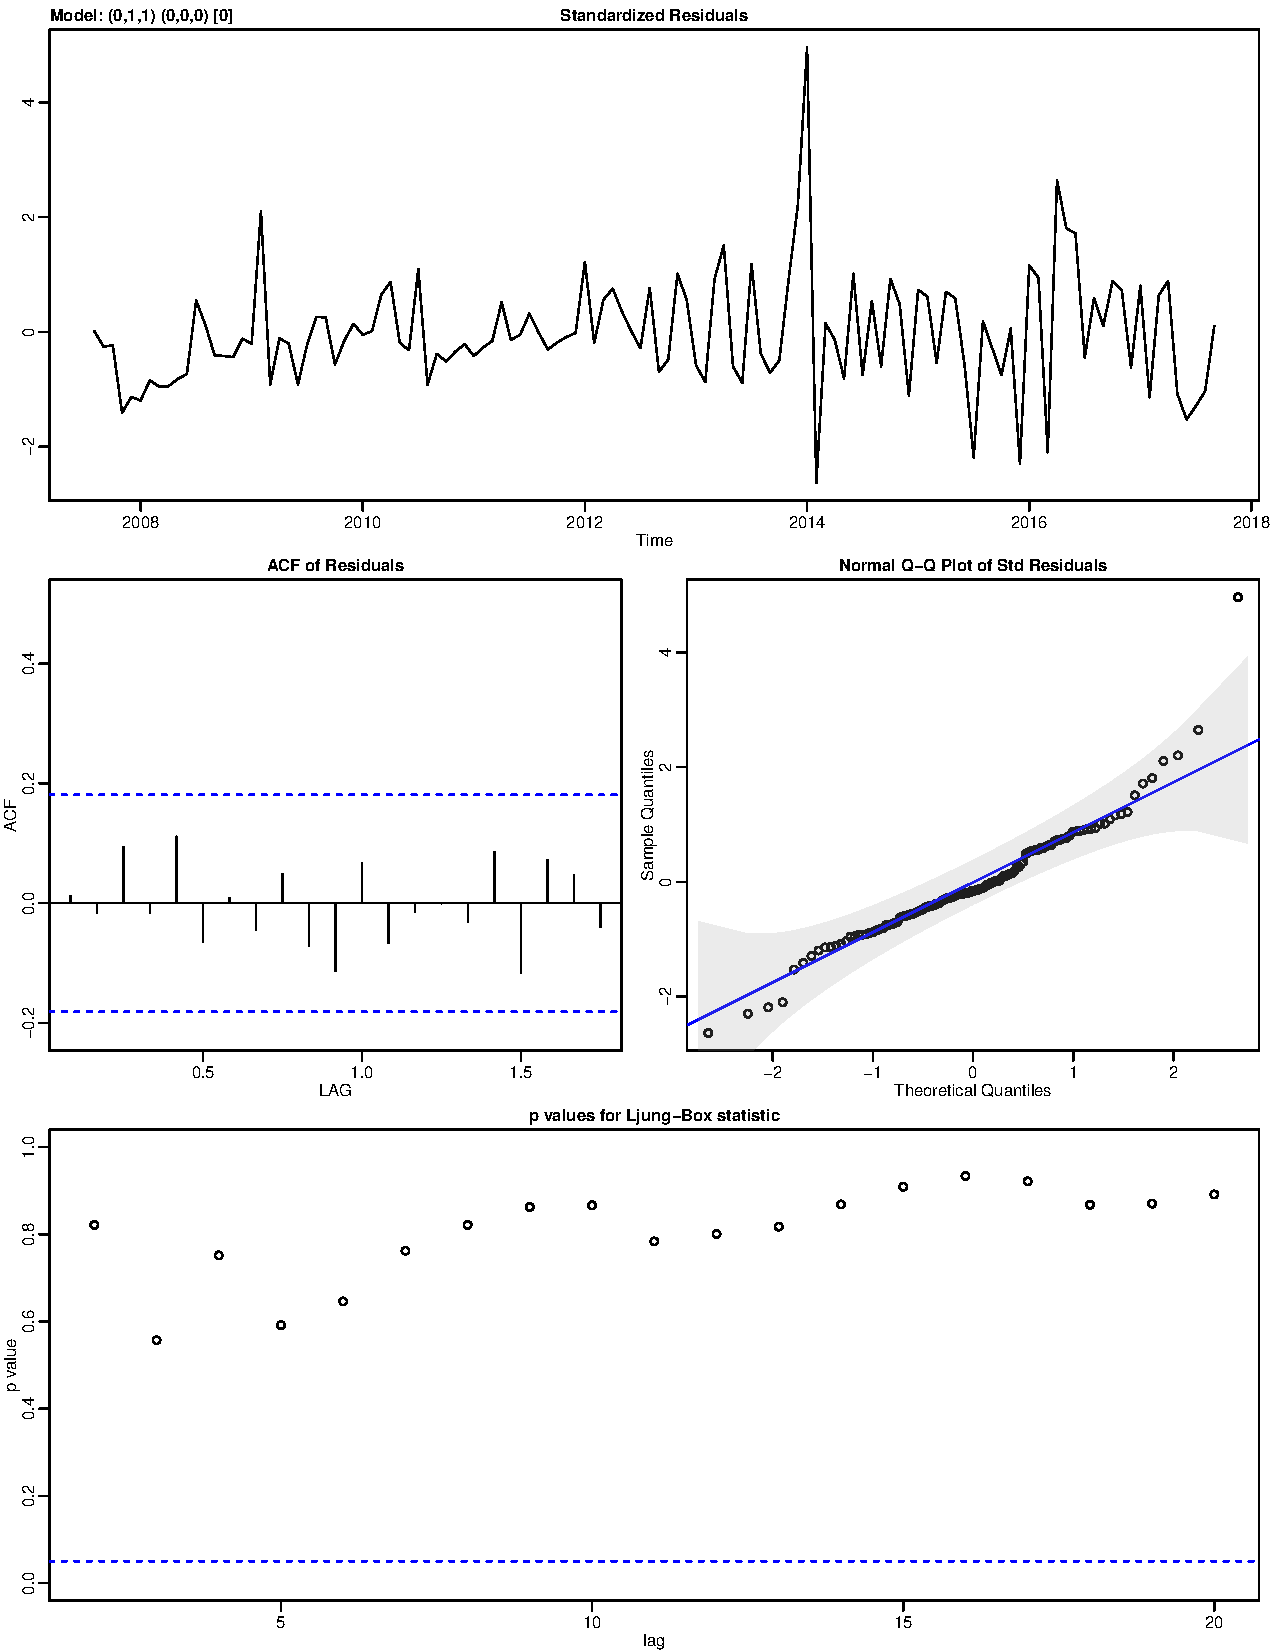
\includegraphics[width=0.6\textwidth]{Sarima_Water_Final}
	\caption{Model Diagnostics , Avg. Watter}
	\label{fig1:Sarima_Water_Final}
\end{figure}

\end{enumerate}
	\newpage
\section{Conclusion}

We arrive at following learning while determining and estimating a model for forecasting time series. 

\begin{enumerate}
	\item Semi-Parametric family of regression worked very well for Avg. Gas and Avg. Water modeling. We have to crossvalidate ($1$ step or $m$ step ahead) to determine the model accuracy. 
	\item ARIMA based modeling works very well when modeling for serially correlated errors as was with Avg. Oil where semi-parametric regression did not do so well. 
	\item ARIMA based approach for modeling all of these processes led to valid and reliable models. We will still need to very forecasts. 
	\item There are elements in the dataset which appear anomalous and not random which gives an intuition of existence of external factors influencing the production of Gas, Water and Oil. 
	\item We had to strip leading $0$ measurements from Avg. Water dataset for estimating and fitting the model. 
	\item We found that running power transform on the data yielded the best results on reduction to white noise with the simplest models on majority of the wells. However, because of issues related to back transformation to original scale we prefer to use ARMA or GAM based models.  
\end{enumerate}

	%% Bibs for citations 

\newpage
\bibliographystyle{plain}
\bibliography{bibfile}
\end{document}